\documentclass[conference]{IEEEtran}
\IEEEoverridecommandlockouts
% The preceding line is only needed to identify funding in the first footnote. If that is unneeded, please comment it out.
\usepackage{cite}
\usepackage{bm,amsbsy,amsmath,amssymb,amsfonts}
\usepackage{algorithmic}
\usepackage{graphicx}
\usepackage{textcomp}
\usepackage[ruled,vlined,linesnumbered]{algorithm2e}
\usepackage{xcolor}
\def\BibTeX{{\rm B\kern-.05em{\sc i\kern-.025em b}\kern-.08em
    T\kern-.1667em\lower.7ex\hbox{E}\kern-.125emX}}
    
\begin{document}

\title{Counting Number of Inversions in an Array\\
{\footnotesize B.tech Semester 4th}
\thanks{}
}

\author{\IEEEauthorblockN{ Harshdeep Singh Pruthi}
\IEEEauthorblockA{\textit{IIT2019105}}
\and
\IEEEauthorblockN{ Jayaram Naik}
\IEEEauthorblockA{\textit{IIT2019106}}
\and
\IEEEauthorblockN{ Shivansh Gupta}
\IEEEauthorblockA{\textit{IIT2019107}}
}

\maketitle

\noindent \begin{abstract}
In this report we have devised an algorithm on how to count the Number of Inversions in an Array.
We have discussed in detail the Divide and Conquer Approach for this problem and discussed why it works and have compared it with the Naive Approach, on what makes it better.
\end{abstract}

\noindent \begin{IEEEkeywords}
Divide and Conquer, Enhanced Merge Sort, Inversions, Sorting
\end{IEEEkeywords}

\section{\textbf{Introduction}}
\noindent Consider an array A, and two indices $\bm{i}$ and $\bm{j}$, such that $\bm{i}<\bm{j}$ and $\bm{A[i]} > \bm{A[j]}$. This is called an inversion in the array. Thus, the Inversion Count of an array is the count of all the pairs $\bm{(i,j)}$ such that $\bm{i}<\bm{j}$ and $\bm{A[i]}>\bm{A[j]}$ \\

\begin{figure}[htbp]
\centerline{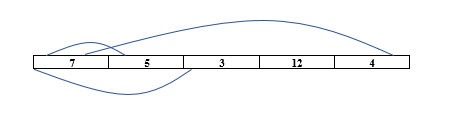
\includegraphics{inversion.png}}
\caption{An example of inversion in array.}
\label{fig}
\end{figure}

\noindent Thus, in the above figure indices $(0,1) , (0,2) , (0,4)$ are called inversions. \\
An important observation here is that Inversion Count can be seen to be closely associated with Sorting of an array. If we find out all the inversions in an array and replace the elements at the indices $\bm{i}$ and $\bm{j}$ to the point that no inversion now exists, the array will be sorted. \\
Thus, Inversion Count for an array indicates – how far the array is from being sorted. If the array is already sorted, then the inversion count is 0, and it would be maximum when the array is sorted in decreasing order. \\
This relationship between inversions and a sorted array is going to be the key for devising a Divide and Conquer algorithm for this problem which shall follow in the subsequent sections.


\section{\textbf{Algorithm Description and Analysis}}

\subsection{Naive}

\noindent The Naive approach is fairly simple. It involves a Brute Force approach where we iterate over all the pairs of the array (which can be done through a nested loop), and if any pair $(i,j)$ satisfies our condition, we increase our Inversion Count by one.

\subsection{Divide and Conquer}
\noindent For the Divide and Conquer approach, suppose we divide our array A into two equal, or almost equal parts. Let's call the first one \textbf{L} and the other one \textbf{R}. Also, let's say we know the Inversion Count of both \textbf{L} and \textbf{R}. Let's call them $\bm{inv_1}$ and $\bm{inv_2}$. \\
Now, suppose we want to count the number of inversions inside the array A. Now any inversion $\bm{(i,j)}$ in \textbf{A} would be of one of the following types: \\

\begin{enumerate}
  \item  $\bm{i \in L}$ and $\bm{j \in R}$.
  \item  $\bm{i \in L}$ and $\bm{j \in L}$.
  \item  $\bm{i \in R}$ and $\bm{j \in R}$.
\end {enumerate}

\begin{itemize}
    \item Let's consider the first case. First of all, it's clear that the total inversions of \textbf{A} now will include the inversions of both \textbf{L} and \textbf{R} ,i.e., $\bm{inv_1} + \bm{inv_2}$. But there may be some more inversions, for when we will $\bm{merge}$ \textbf{L} and \textbf{R}. And that is the major step in this case - computing for each index $\bm{i \in L}$, the number of indices $\bm{j \in R}$ such that L\textsubscript i $>$ R\textsubscript j.\\
    Now, let's say that we have sorted the arrays \textbf{L} and \textbf{R}. and their sizes are \textbf{N} and \textbf{M} respectively. \\
    Also, now consider we are using $\bm{k}$ and $\bm{l}$ to iterate over \textbf{L} and \textbf{R}. Say, at certain point we encounter $\bm{L[l]} > \bm{R[k]}$.\\
    Now, because \textbf{L} and \textbf{R} are sorted, we know that there are going to be \textbf{N-i} more inversions in \textbf{A}, because all elements to the right of $\bm{L[l]}$ will also be greater than $\bm{R[k]}$.\\
    Note that it doesn't matter that the elements are now sorted, because all the elements of \textbf{L} existed to the left of all elements \textbf{R} in the original array \textbf{A}, so these inversions will be present in one or another order in \textbf{A}.
    \\
    \item Now for the second and the third case: If we encounter that situation, we again divide them up into further two arrays and repeat this recursively, until we have arrived on the base case - that includes just one element. And in this case, we know the inversions will be $0$, because there is just a single element in the array.
\end{itemize}

Here, one more important thing is that in the first case, we require the arrays \textbf{L} and \textbf{R} to be sorted. To achieve that, the algorithm must sort them. In other words, after applying the algorithm to both L and R, they become sorted. To sort \textbf{A} we just merge the two sorted arrays \textbf{L} and \textbf{R} into \textbf{A}.

\section{\textbf{Pseudo Code}}
\begin{algorithm}
\While{$i < N$}{
    \While{$j < N$}{
        \If{$i< j$ AND $A[i] > A[j]$}{
            increment invCount\\
            increment j
        }
    }
    increment i
}
\caption{Naive Approach}
\end{algorithm}
\noindent \textbf{Divide and Conquer Approach}\\
\noindent We will be creating two functions: \textbf{enhancedMergeSort} and \textbf{mergeTwoArrays}. The former will divide up the array recursively into halves and call the latter function for these divided arrays and the latter function will sort the arrays and in the process return the Inversion Count which is ultimately added up to return the final answer.


\begin{algorithm}
\DontPrintSemicolon

    \KwData{$\bm{arr}$: The Array\\
         $\bm{beg}$: Start iterator\\
         $\bm{mid}$: Middle iterator\\
         $\bm{end}$: End iterator\\}
  \KwResult{Returns the total number of inversions in the procedure of merging two arrays $\bm{arr[beg...mid]}$ and $\bm{arr[mid+1...end]}$}
  $i,k=beg$\\
  $j=end$\\
  $newarr$\\
  \While{$i<mid$ AND $j<=end$}
  {
    \tcc{No Inversion}
    \If{$arr[i]<arr[j]$}
    {
        newarr[k]=arr[i]\\
        increment k,i
    }
    \tcc{mid-i inversions}
    \Else{
        newarr[k]=arr[j]\\
        invCount+= $mid-i$\\
        increment k,j
    }
  }
  \While{$i<mid$}{
    temp[k] = arr[i]\\
    increment k,i
  }
  \While{$j,end$}{
    temp[k] = arr[j]\\
    increment k,j
  }
  it = beg
\tcc{Copy all the elements of newarr into arr}
  \While{$it < end$}{
    arr[it] = newarr[it]
    increment it
  }
  return $invCount$
\caption{mergeTwoArrays}
\end{algorithm}

\begin{algorithm}
\DontPrintSemicolon
  
  \KwData{$\bm{arr}$: The Array\\
         $\bm{beg}$: Start iterator\\
         $\bm{end}$: End iterator\\}
  \KwResult{Returns the total number of inversions in the array arr from $\bm{beg}$ to $\bm{end}$}
  $mid, invCount=0$\\
  \If{$end>beg$}
    {
        mid = (beg+end)/2
        
        \tcc{Call recursively and add returned value to invCount}
        invCount += enhancedMergeSort(arr,left,mid)\\
        invCount += enhancedMergeSort(arr,mid+1,right)
        \\
        \tcc{Merge these arrays up using the merge function which also returns the inversion count of the process}
        invCount += mergeTwoArrays(arr,left,mid+1,right)
    }
    
    return $invCount$\\
\caption{enhancedMergeSort}
\end{algorithm}

\section{\textbf{Complexity Analysis}}
\subsection{Time complexity}
\noindent In the \textbf{Naive Approach}, for any index $\bm{i}$, there are \textbf{N-i} iterations. Thus the total number of iterations will be the sum of \textbf{N,N-1,N-2,...1}, thus making the Time Complexity of theorder of O($N^2$).\\
In the \textbf{Divide and Conquer} algorithm , the input array is divided into two halves each time it is processed.
As such it can be expressed with following recurrence relation,
\begin{center} T(n) = 2T(n/2) + $\theta$(n).\end{center}
Now assuming that at each step the array is divided into exactly two halves, the maximum depth we will get will be $log_2(N)$\\
Hence, time complexity for the same is \begin{center} \textbf{O(Nlog(N))} \end{center}
\begin{figure}[htbp!]
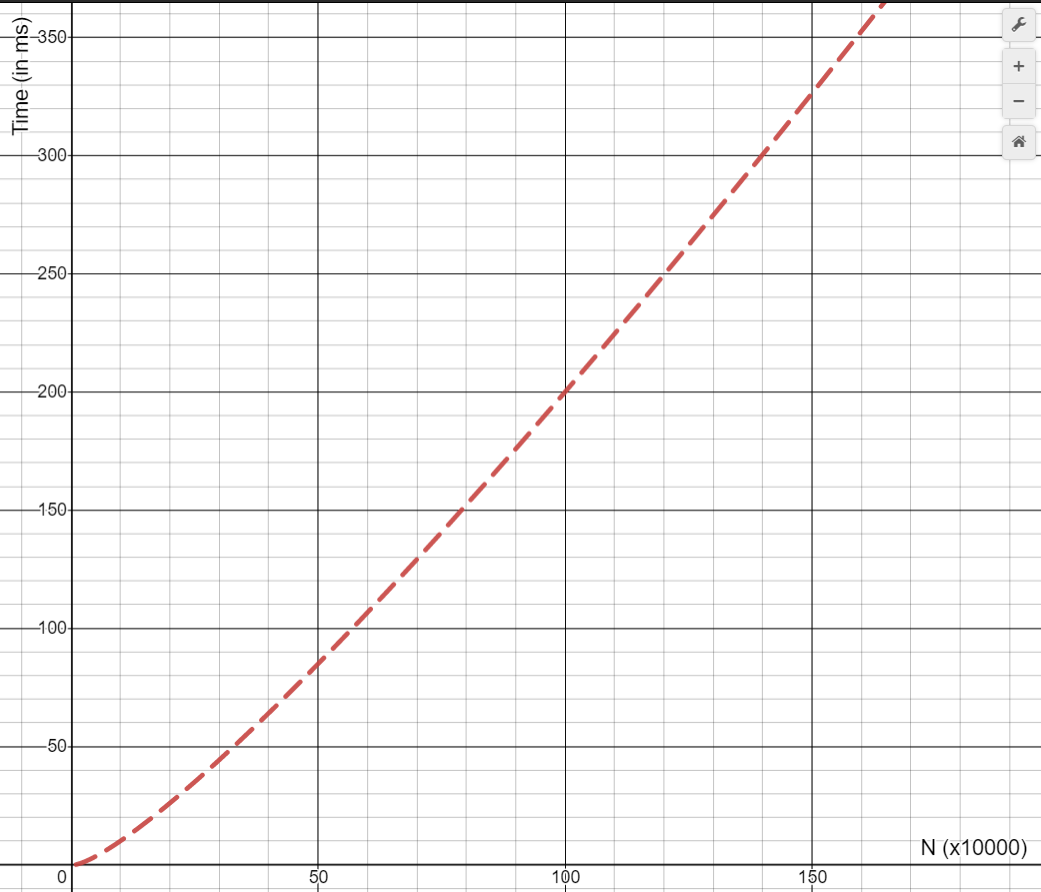
\includegraphics[width=0.5\textwidth]{timeComplexity.png}
\caption{Time Complexity : O(Nlog(N))}
\label{Time Complexity}
\end{figure}

\subsection{Space complexity}
\noindent In the \textbf{Divide and Conquer} algorithm, in process of counting inversions, we are also sorting the input array as the algorithm demands this. If we wish to retain the original array we do need an auxiliary array which is the copy of the input array .\\ Thus, the space complexity will be O(N) .\\
The space complexity of \textbf{Naive Approach} would also be O(N). But it must be noted that in actual practice the spaced used by Naive Approach would be slightly less than that used by the Divide and Conquer Approach because although its order is still O(N), the Recursive calls do fill up the Function's memory stack\\
\begin{figure}[htbp]
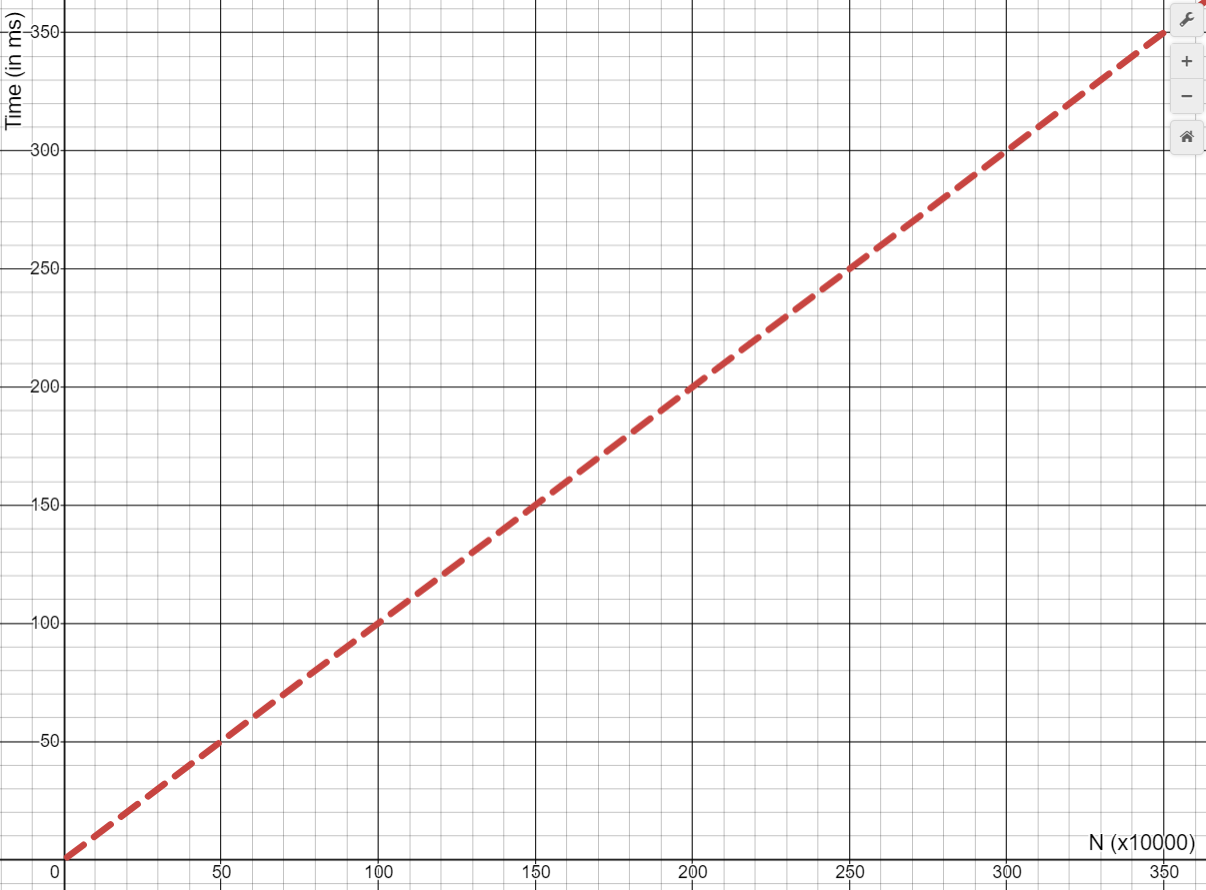
\includegraphics[width=0.5\textwidth]{spaceComplexity.png}
\caption{Space Complexity : O(N)}
\label{Space Complexity}
\end{figure}

\begin{thebibliography}{00}
\bibitem{b1}{Introduction to Algorithms by Thomas H. Cormen, Charles E. Leiserson, Ronald Rivest, Clifford Stein}\\
\bibitem{b2}{Introduction to Design and Analysis of Algorithms by Anany Levitin}\\
\bibitem{b3}{Algorithms by Robert Sedgewick and Kevin Wayne}
\end{thebibliography}
\vspace{12pt}

\end{document}